\section{Appendix}\label{section:appendix}

% ---------- Part A ----------
\subsection*{Part A: Single-qubit gates and measurements}

\begin{figure}[H]
    \centering
    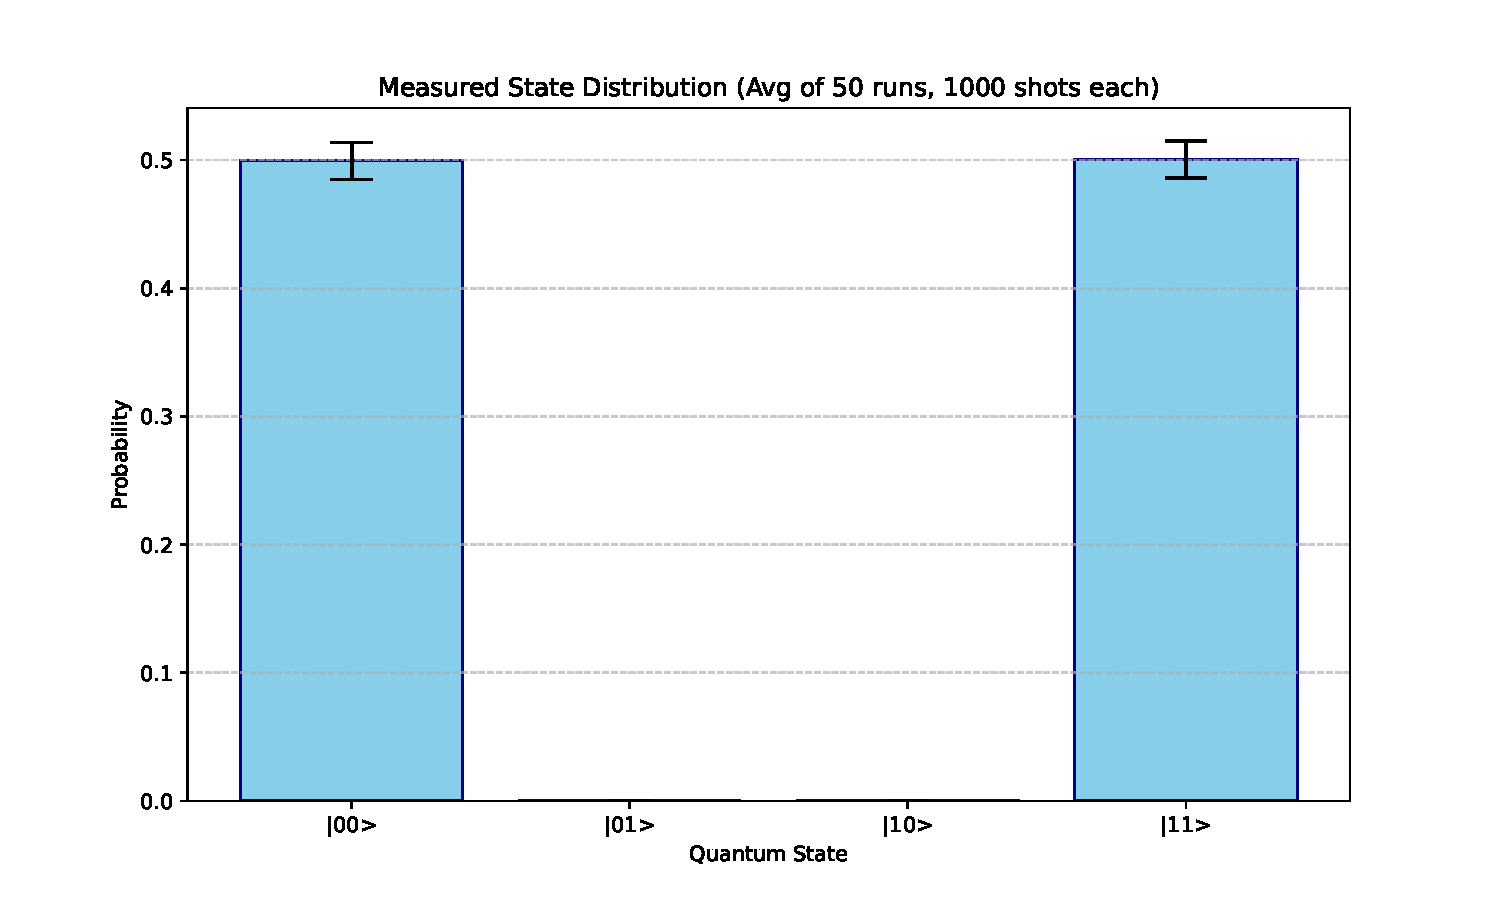
\includegraphics[width=0.78\textwidth]{figures/part-a_measurement_dist.pdf}
    \caption{Measurement outcome distribution.}
    \label{fig:app_a_measdist}
\end{figure}

% \clearpage

% ---------- Part B ----------
\subsection*{Part B: Two-level model (exact diagonalization)}

\begin{figure}[H]
\centering
\begin{subfigure}[t]{0.4\textwidth}
\centering
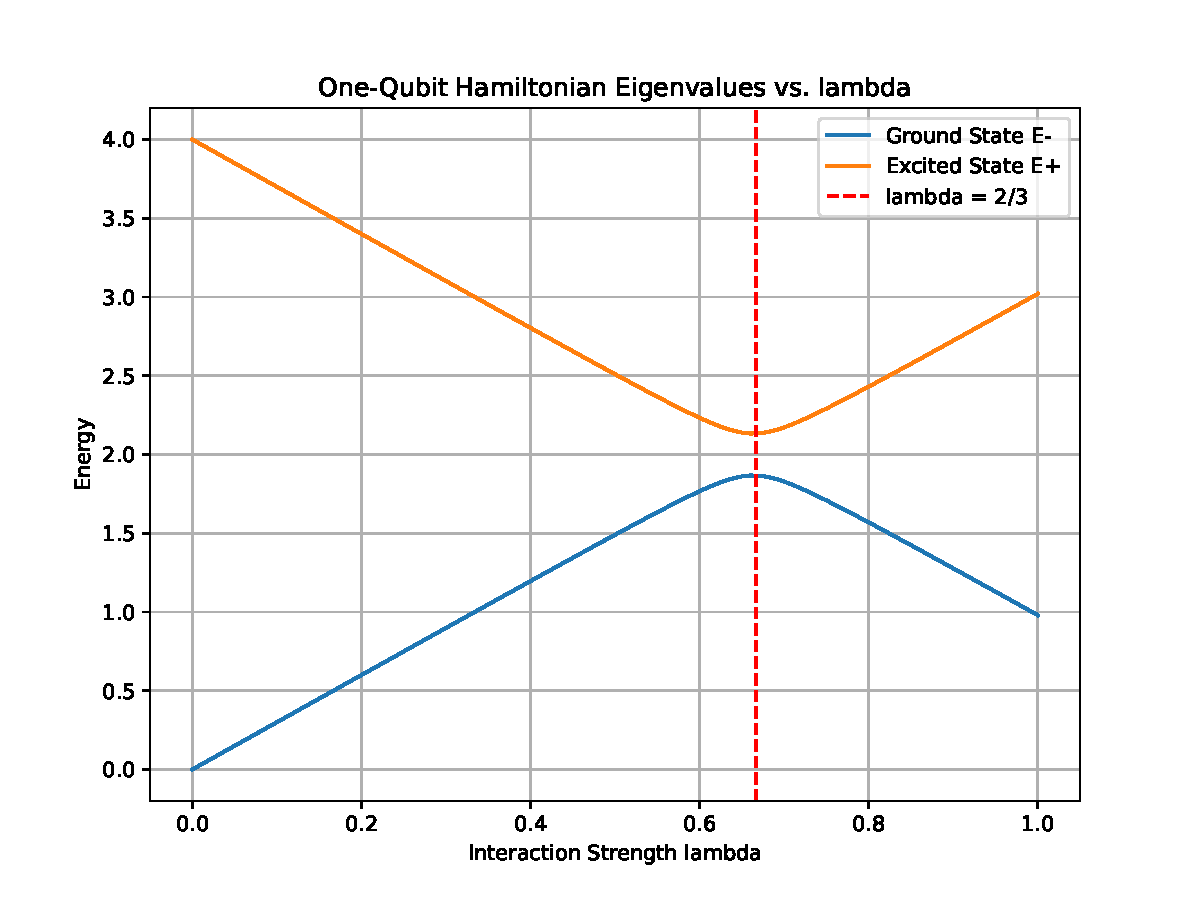
\includegraphics[width=\linewidth]{figures/part-b_eigenvalues.pdf}
\caption{Eigenvalues vs.\ $\lambda$.}
\label{fig:app_b_eigs}
\end{subfigure}
\hfill
\begin{subfigure}[t]{0.4\textwidth}
\centering
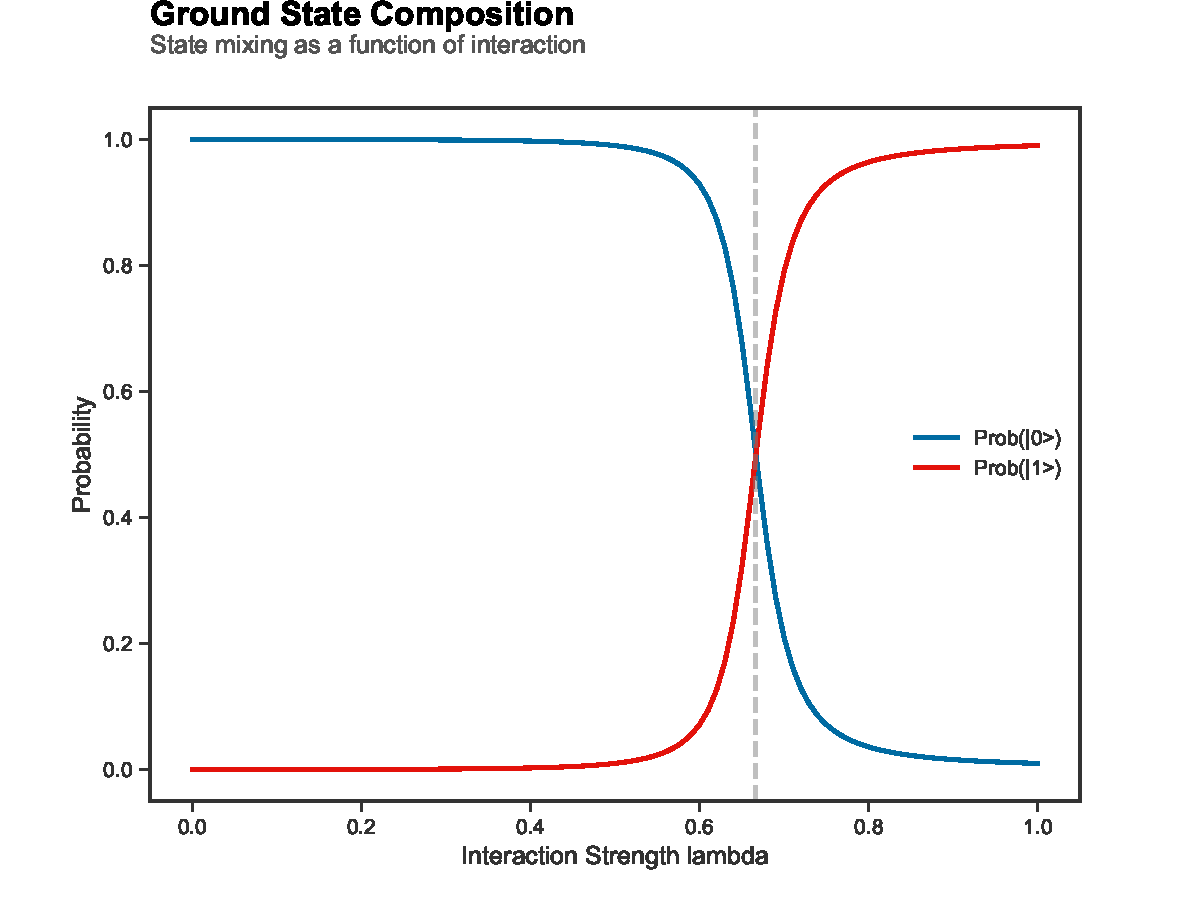
\includegraphics[width=\linewidth]{figures/part-b_eigenvector_mixing.pdf}
\caption{Eigenvector mixing.}
\label{fig:app_b_mix}
\end{subfigure}
\caption{Exact spectrum and state character for the $2\times2$ Hamiltonian.}
\label{fig:app_b}
\end{figure}

% \clearpage

% ---------- Part C ----------
\subsection*{Part C: VQE for the two-level model}

\begin{figure}[H]
\centering
\begin{subfigure}[t]{0.4\textwidth}
\centering
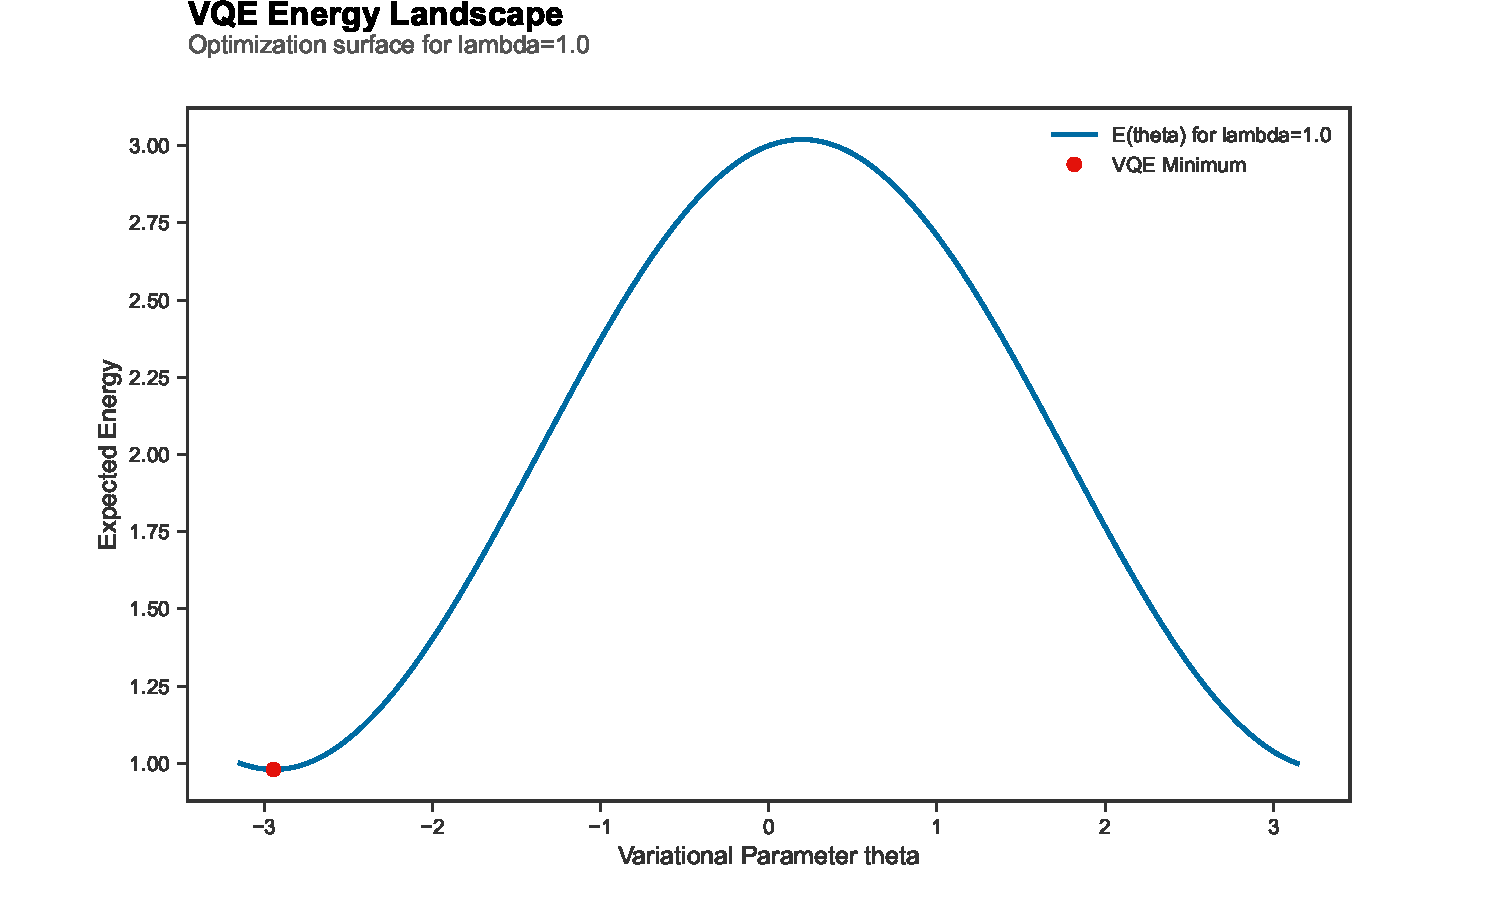
\includegraphics[width=\linewidth]{figures/part-c_energy_landscape.pdf}
\caption{Energy landscape.}
\label{fig:app_c_landscape}
\end{subfigure}
\hfill
\begin{subfigure}[t]{0.4\textwidth}
\centering
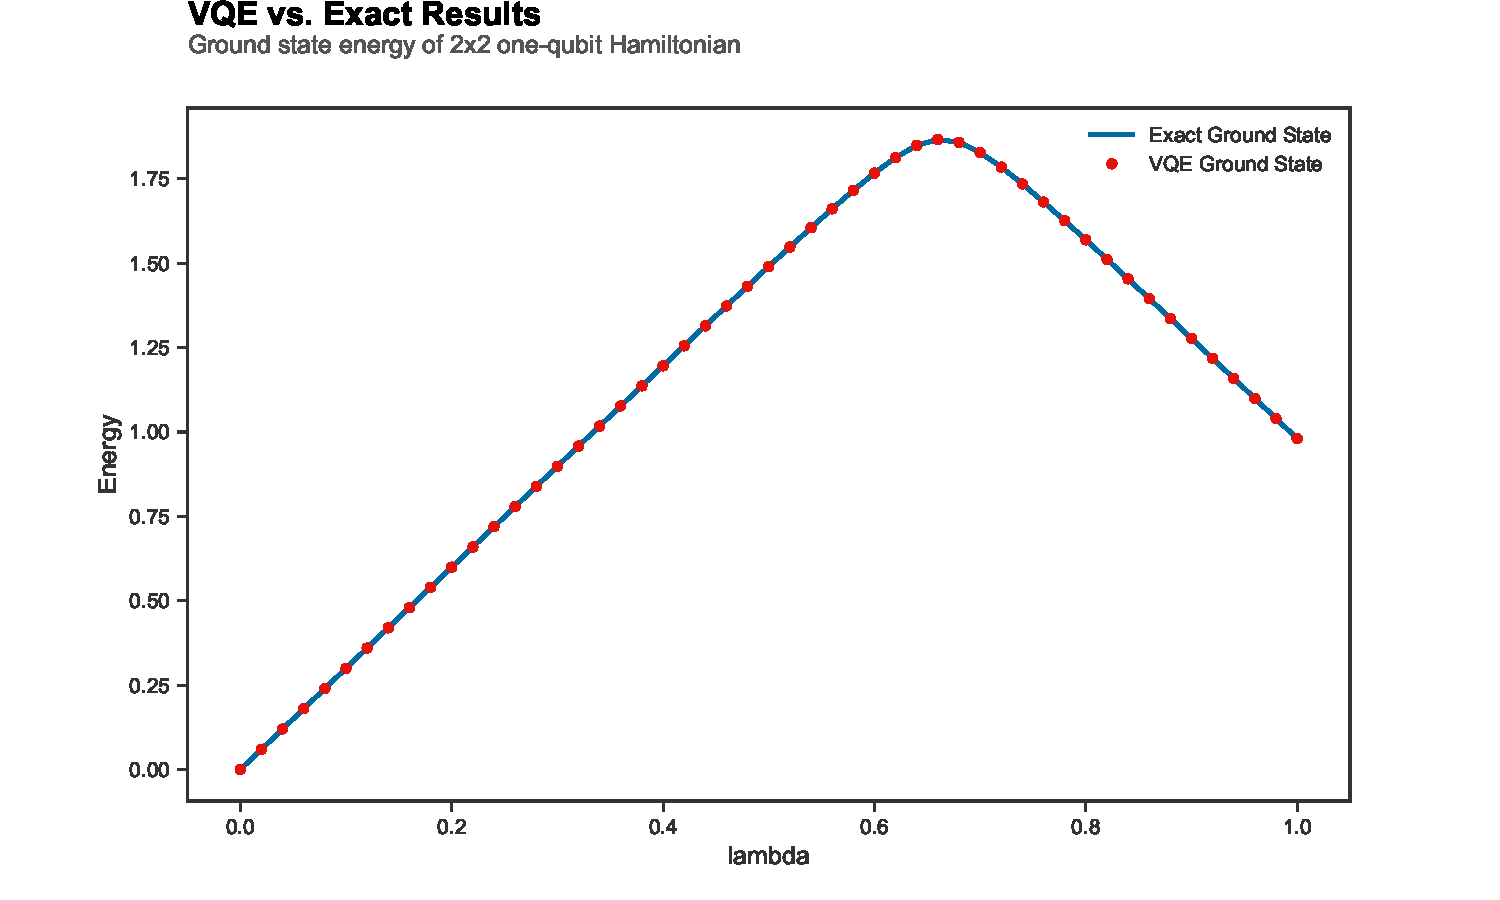
\includegraphics[width=\linewidth]{figures/part-c_vqe_comp.pdf}
\caption{VQE vs.\ exact.}
\label{fig:app_c_comp}
\end{subfigure}

\vspace{0.6em}

\begin{subfigure}[t]{0.4\textwidth}
\centering
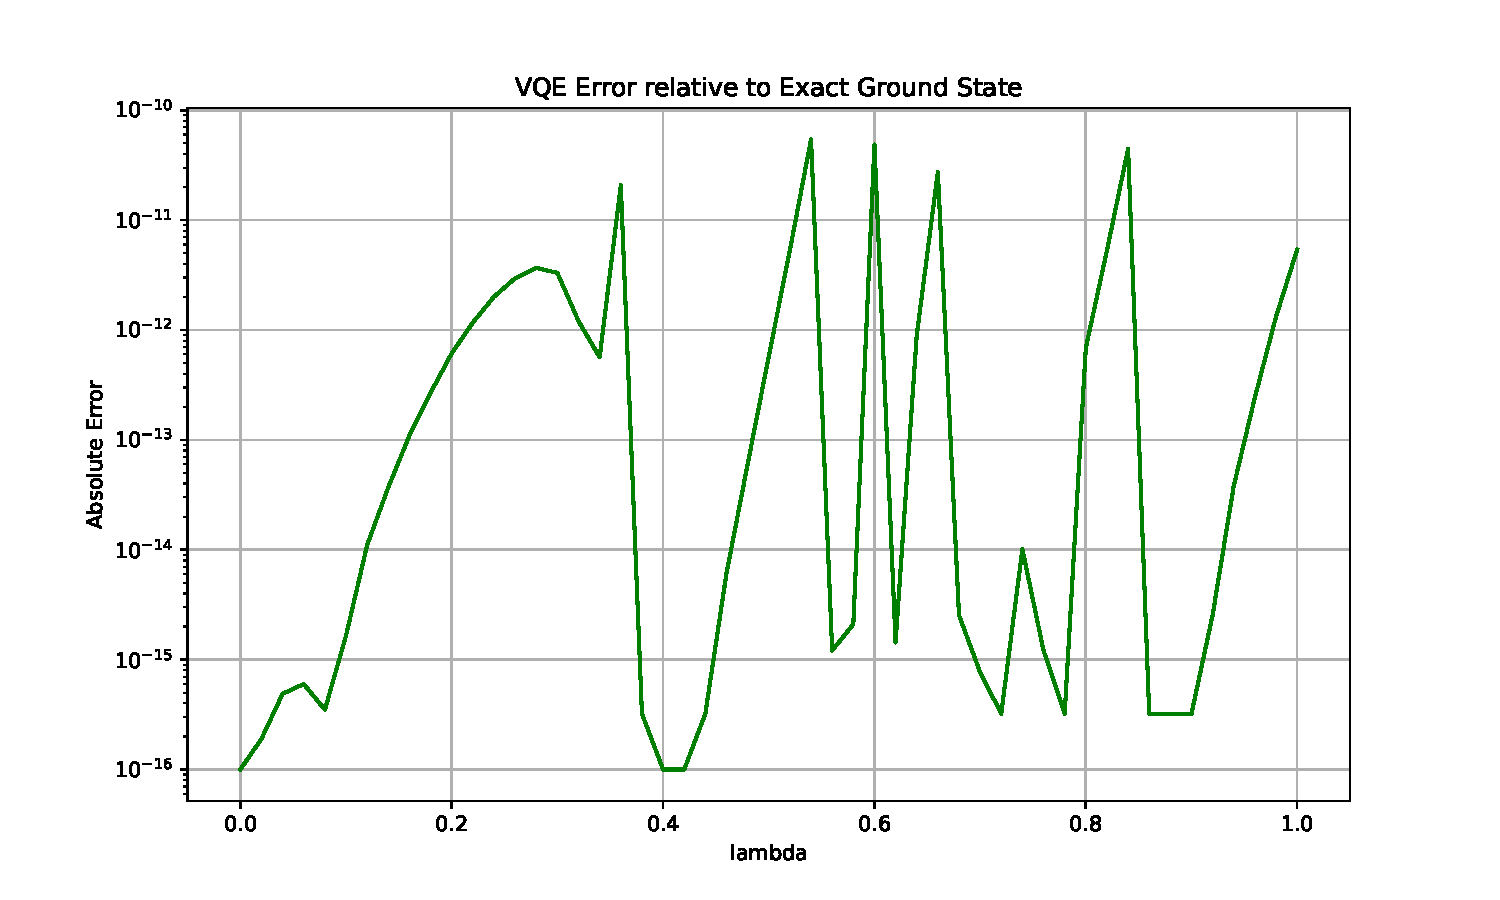
\includegraphics[width=\linewidth]{figures/part-c_vqe_error.pdf}
\caption{Absolute error.}
\label{fig:app_c_err}
\end{subfigure}
\hfill
\begin{subfigure}[t]{0.4\textwidth}
\centering
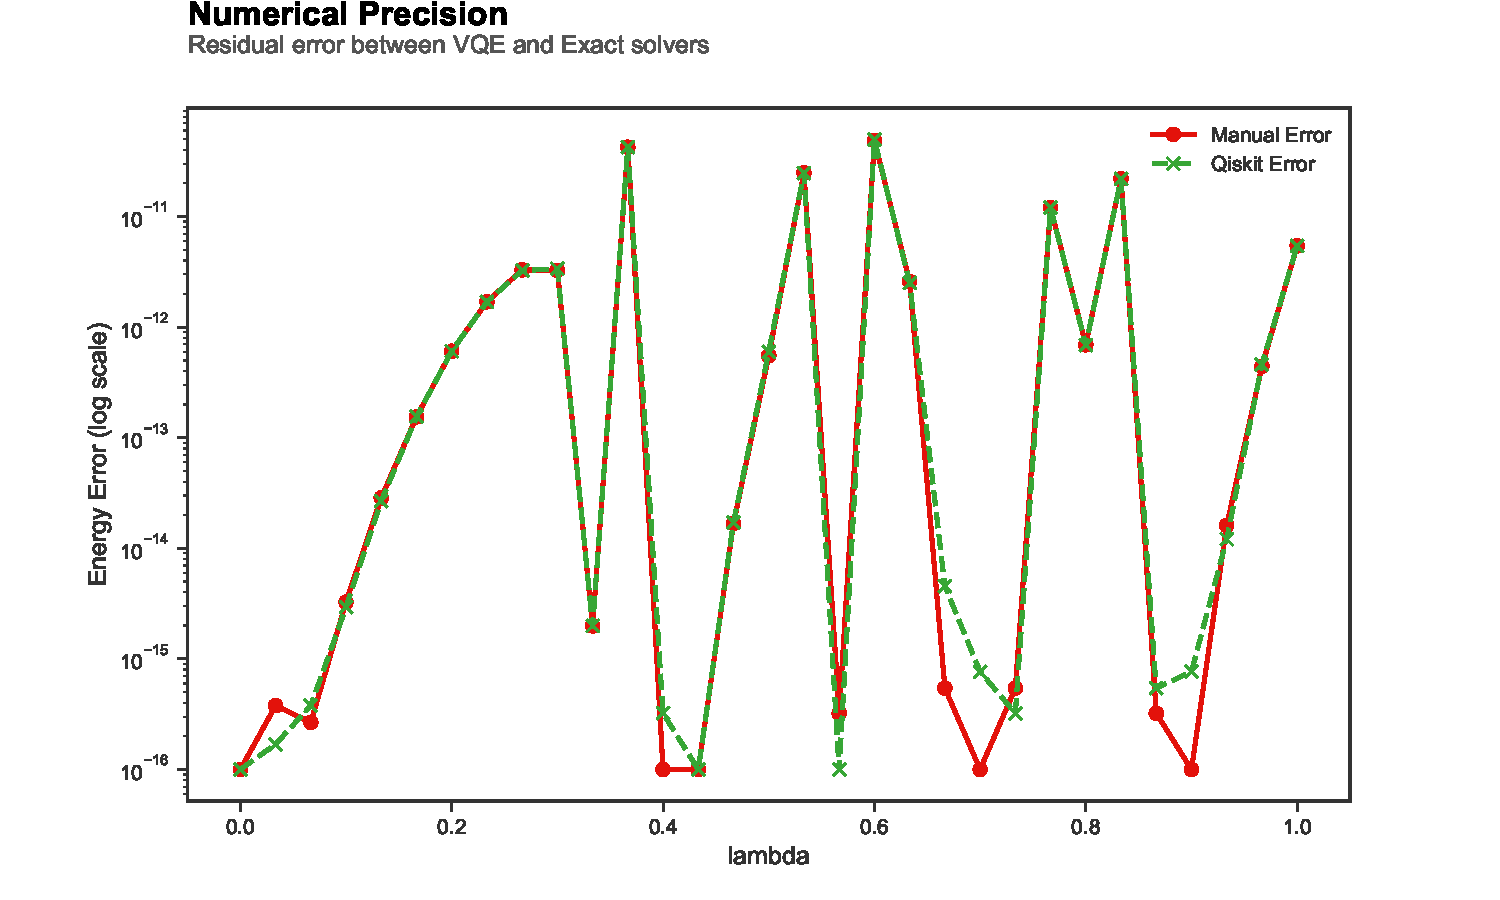
\includegraphics[width=\linewidth]{figures/part-c_vqe_precision.pdf}
\caption{Precision.}
\label{fig:app_c_prec}
\end{subfigure}
\caption{VQE optimization diagnostics for the $2\times2$ model.}
\label{fig:app_c_opt}
\end{figure}

% \clearpage

\begin{figure}[H]
\centering
\begin{subfigure}[t]{0.4\textwidth}
\centering
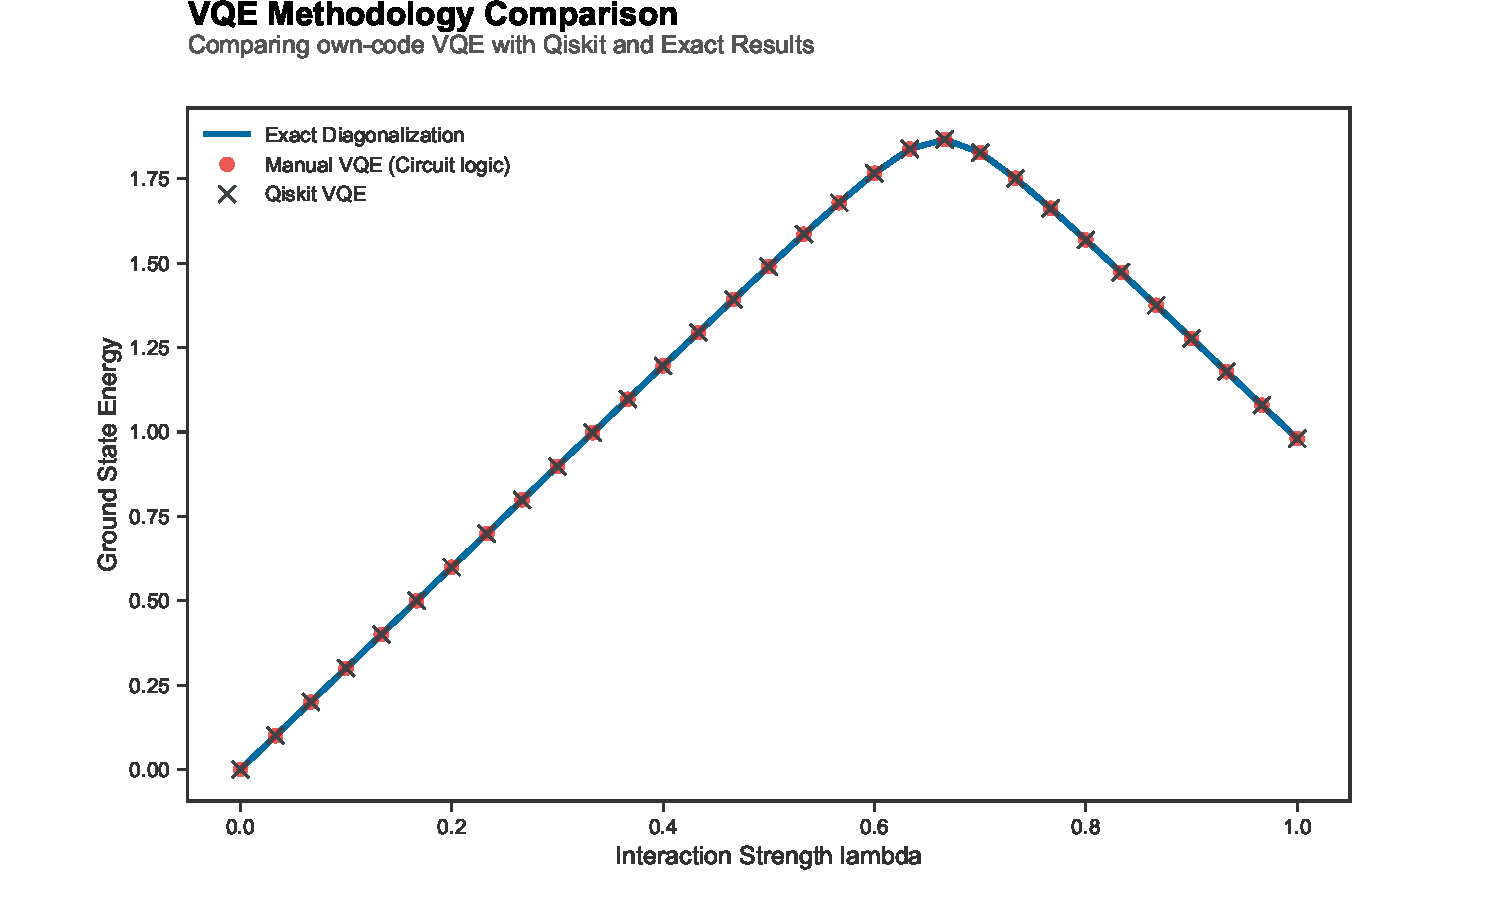
\includegraphics[width=\linewidth]{figures/part-c_vqe_method_comparison.pdf}
\caption{Method comparison.}
\label{fig:app_c_methods}
\end{subfigure}
\hfill
\begin{subfigure}[t]{0.4\textwidth}
\centering
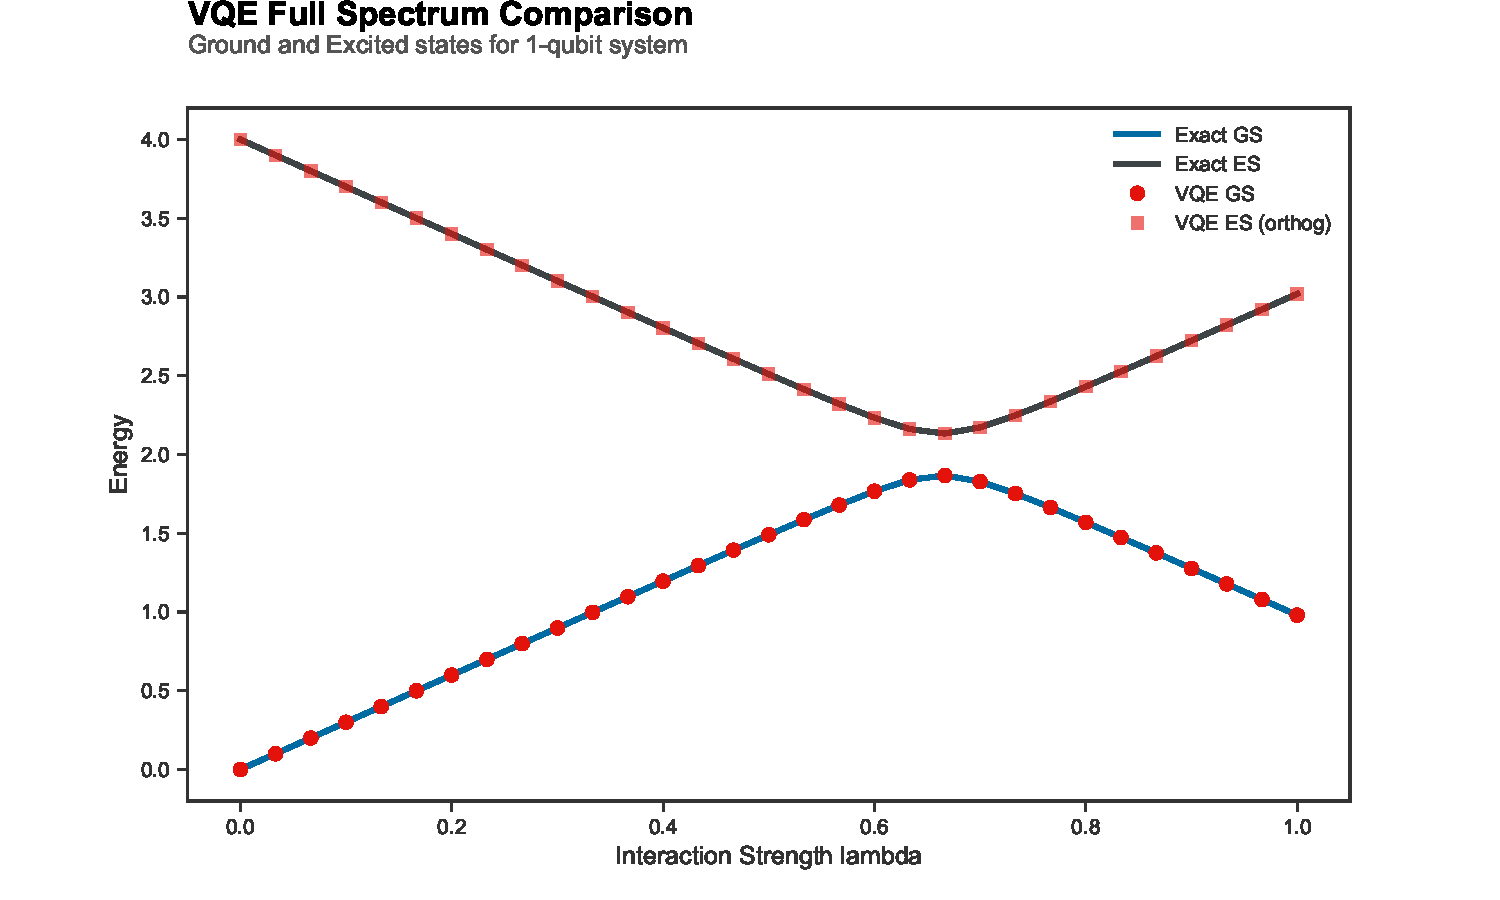
\includegraphics[width=\linewidth]{figures/part-c_vqe_full_spectrum.pdf}
\caption{Full spectrum.}
\label{fig:app_c_fullspec}
\end{subfigure}

\vspace{0.6em}

\begin{subfigure}[t]{0.4\textwidth}
\centering
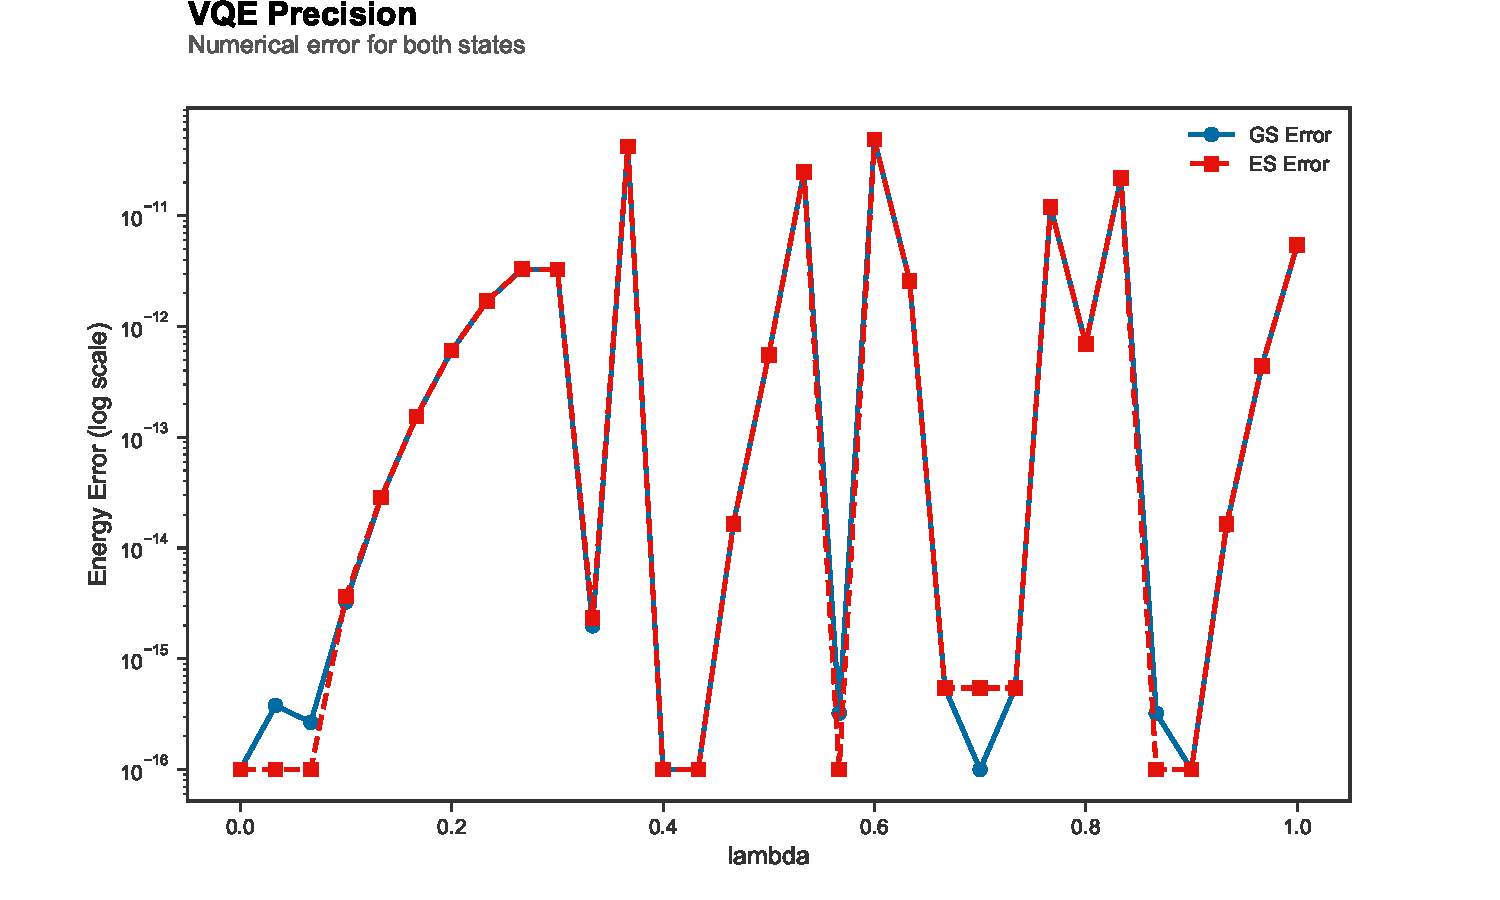
\includegraphics[width=\linewidth]{figures/part-c_vqe_spectrum_error.pdf}
\caption{Spectrum error.}
\label{fig:app_c_specerr}
\end{subfigure}
\caption{Spectrum-level VQE comparisons for the $2\times2$ model.}
\label{fig:app_c_spec}
\end{figure}

% \clearpage

% ---------- Part D ----------
\subsection*{Part D: Two-qubit model and entanglement}

\begin{figure}[H]
\centering
\begin{subfigure}[t]{0.4\textwidth}
\centering
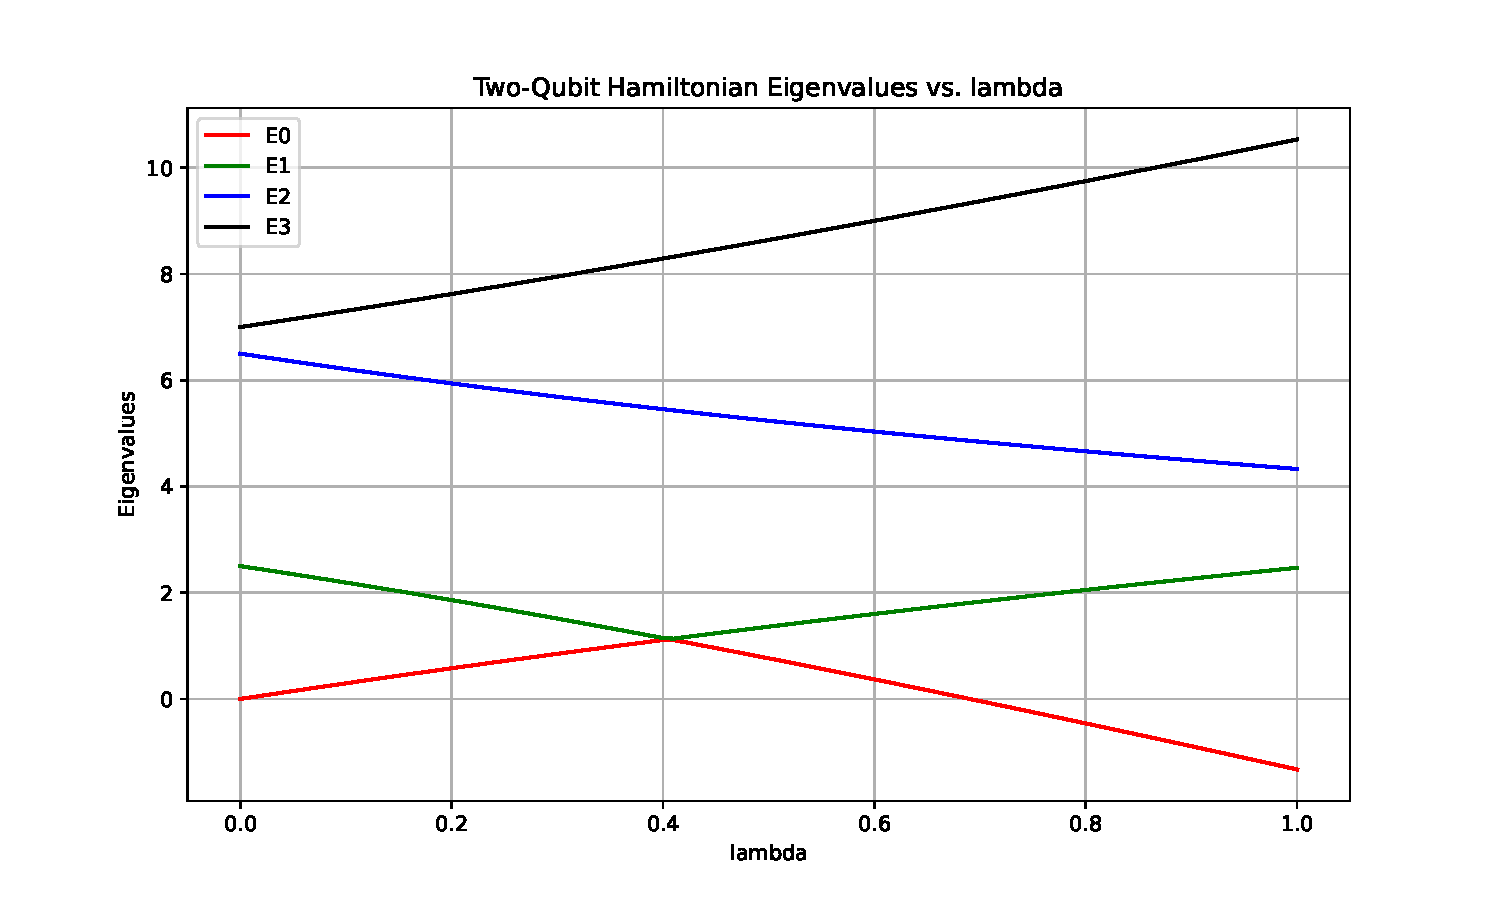
\includegraphics[width=\linewidth]{figures/part-d_eigenvalues.pdf}
\caption{Eigenvalues vs.\ $\lambda$.}
\label{fig:app_d_eigs}
\end{subfigure}
\hfill
\begin{subfigure}[t]{0.4\textwidth}
\centering
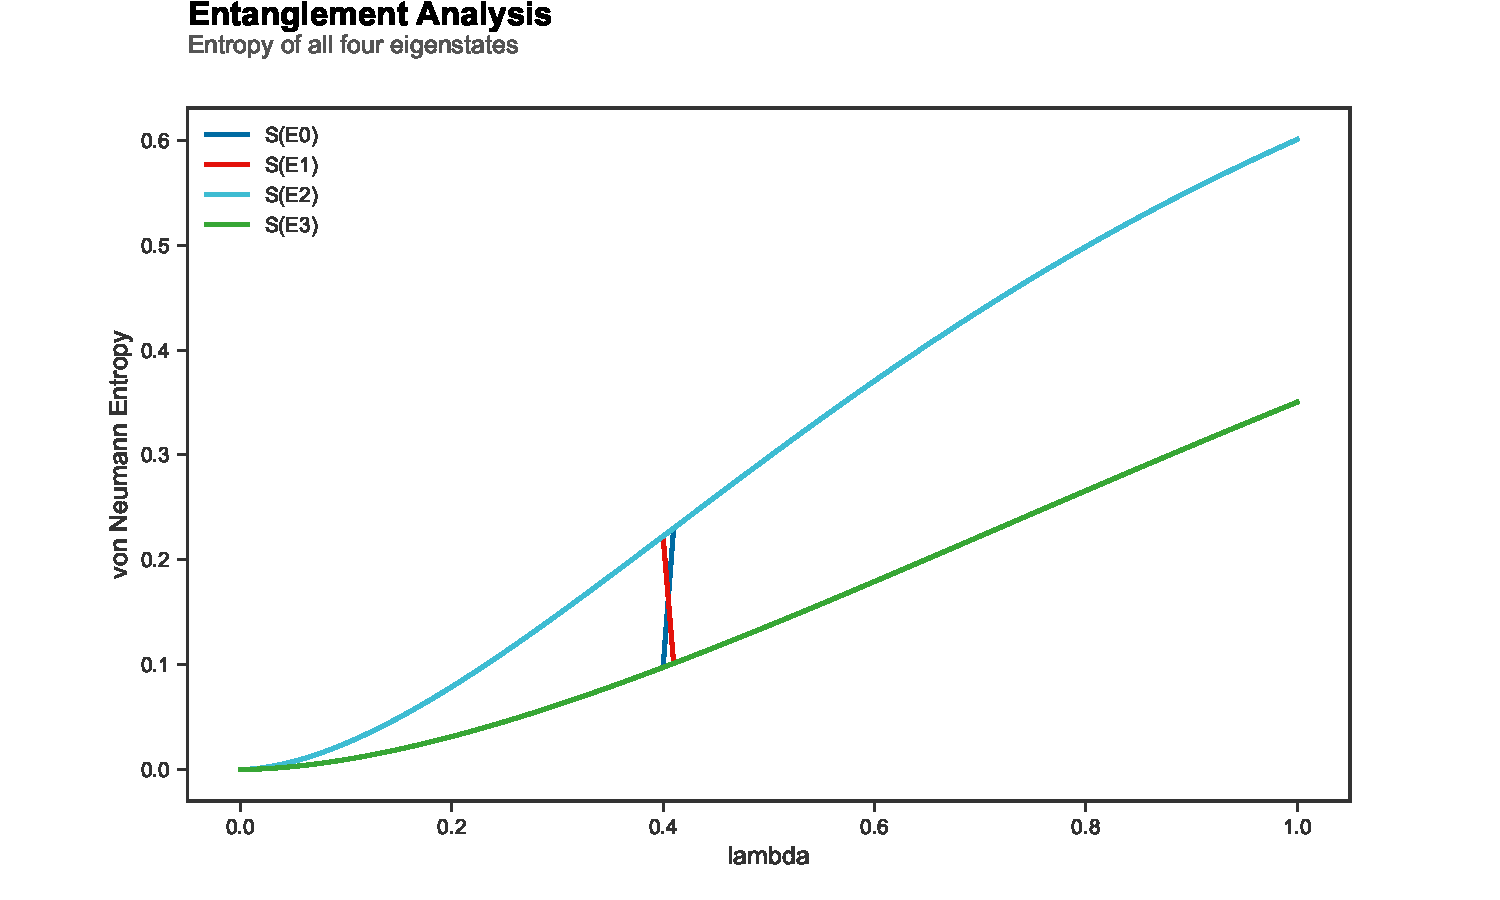
\includegraphics[width=\linewidth]{figures/part-d_entropy.pdf}
\caption{Von Neumann entropy.}
\label{fig:app_d_entropy}
\end{subfigure}
\caption{Spectrum and entanglement diagnostics for the two-qubit Hamiltonian.}
\label{fig:app_d}
\end{figure}

% \clearpage

% ---------- Part E ----------
\subsection*{Part E: VQE for the two-qubit model}

\begin{figure}[H]
\centering
\begin{subfigure}[t]{0.4\textwidth}
\centering
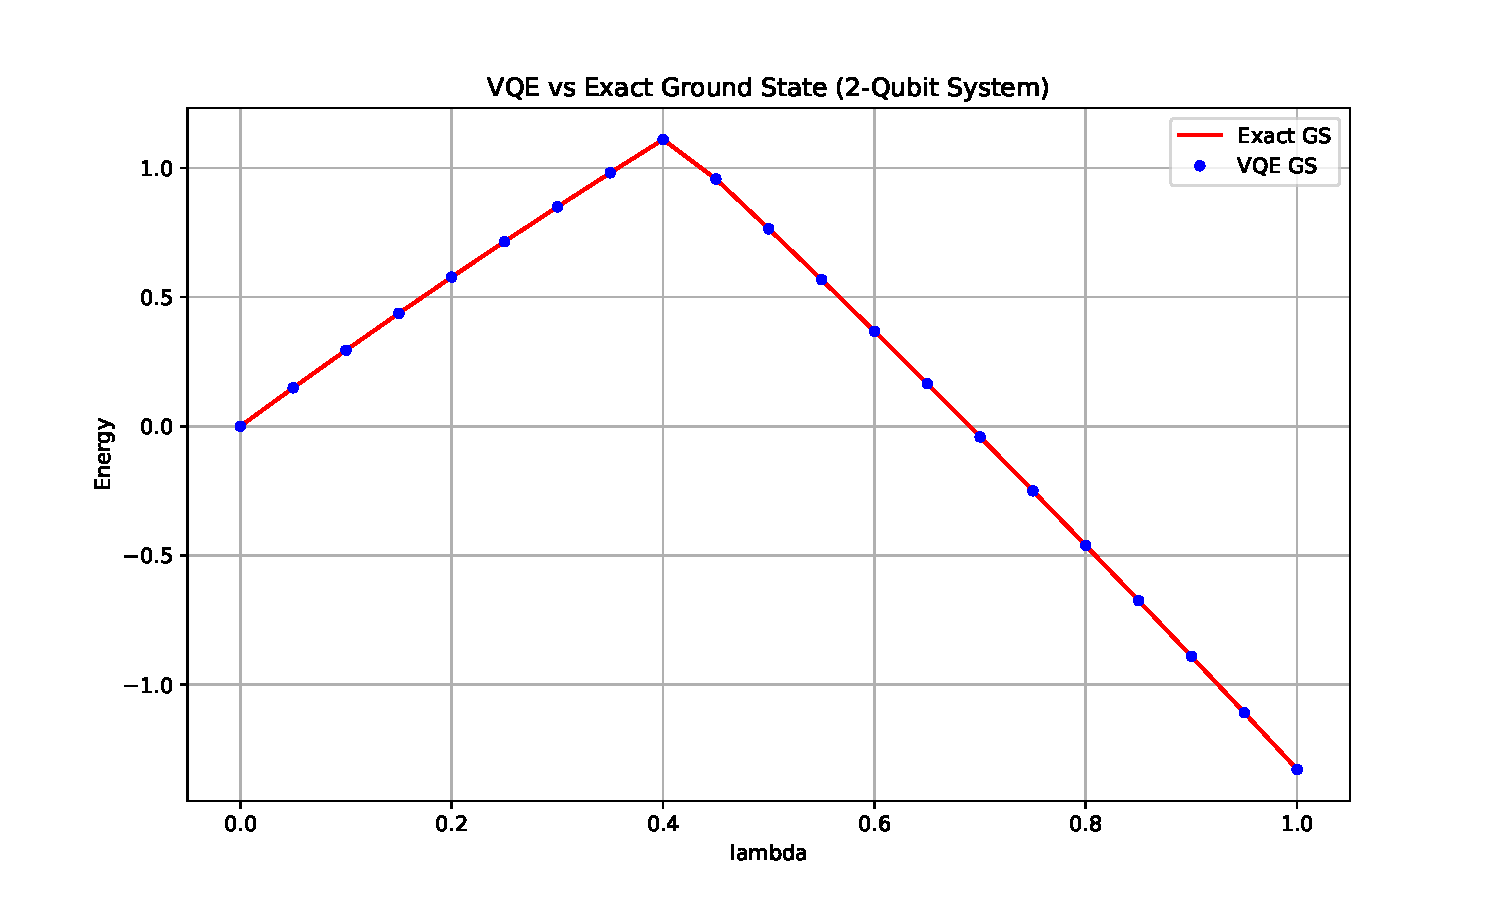
\includegraphics[width=\linewidth]{figures/part-e_vqe_comp.pdf}
\caption{VQE vs.\ exact.}
\label{fig:app_e_comp}
\end{subfigure}
\hfill
\begin{subfigure}[t]{0.4\textwidth}
\centering
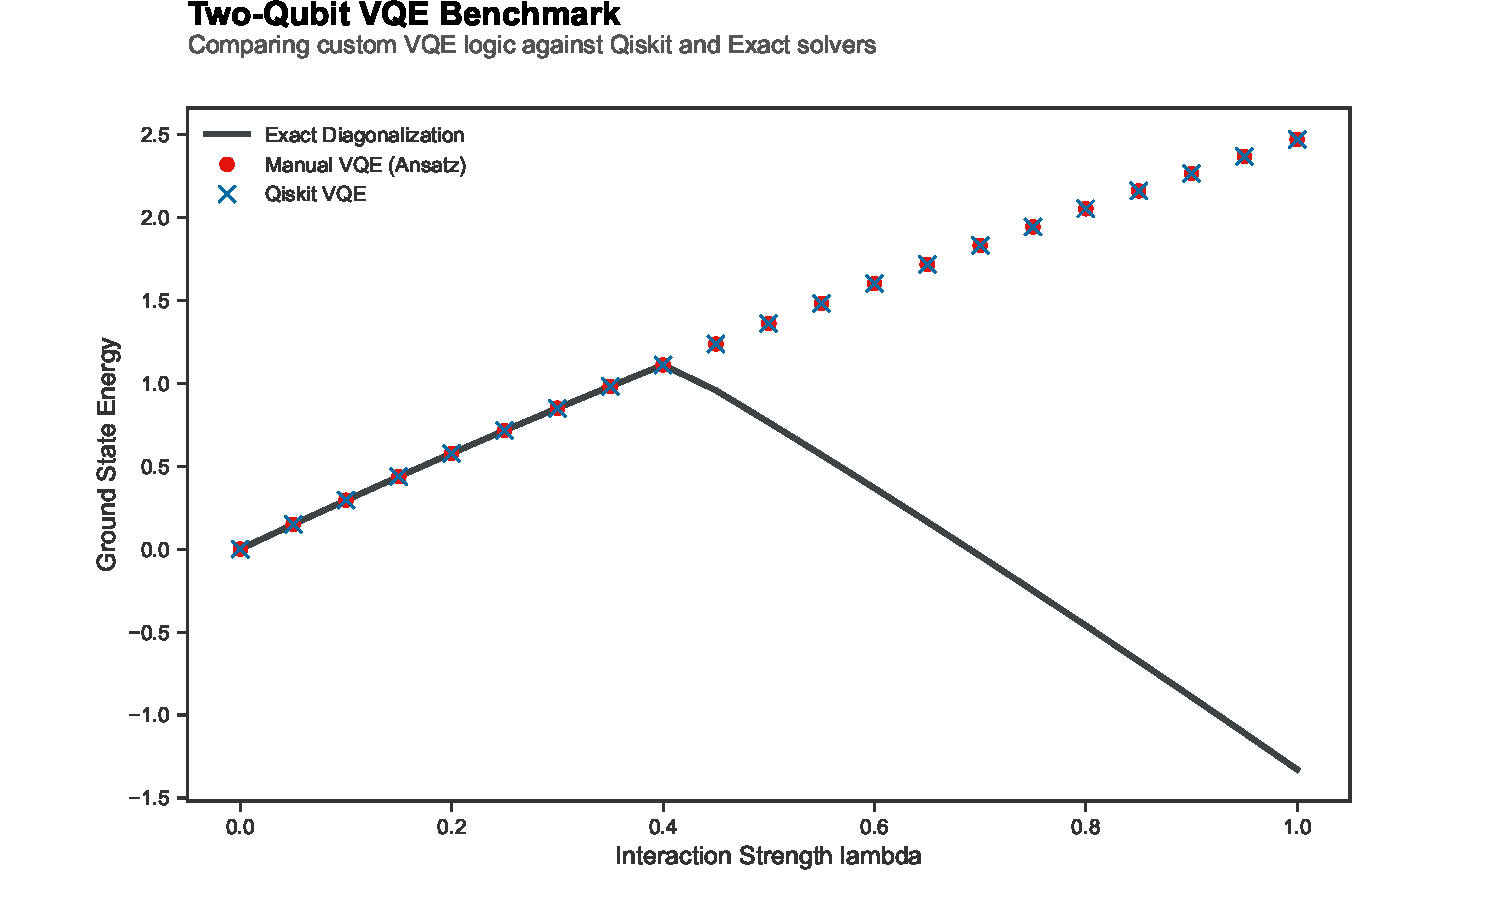
\includegraphics[width=\linewidth]{figures/part-e_vqe_comparison.pdf}
\caption{Comparison.}
\label{fig:app_e_compare}
\end{subfigure}

\vspace{0.6em}

\begin{subfigure}[t]{0.4\textwidth}
\centering
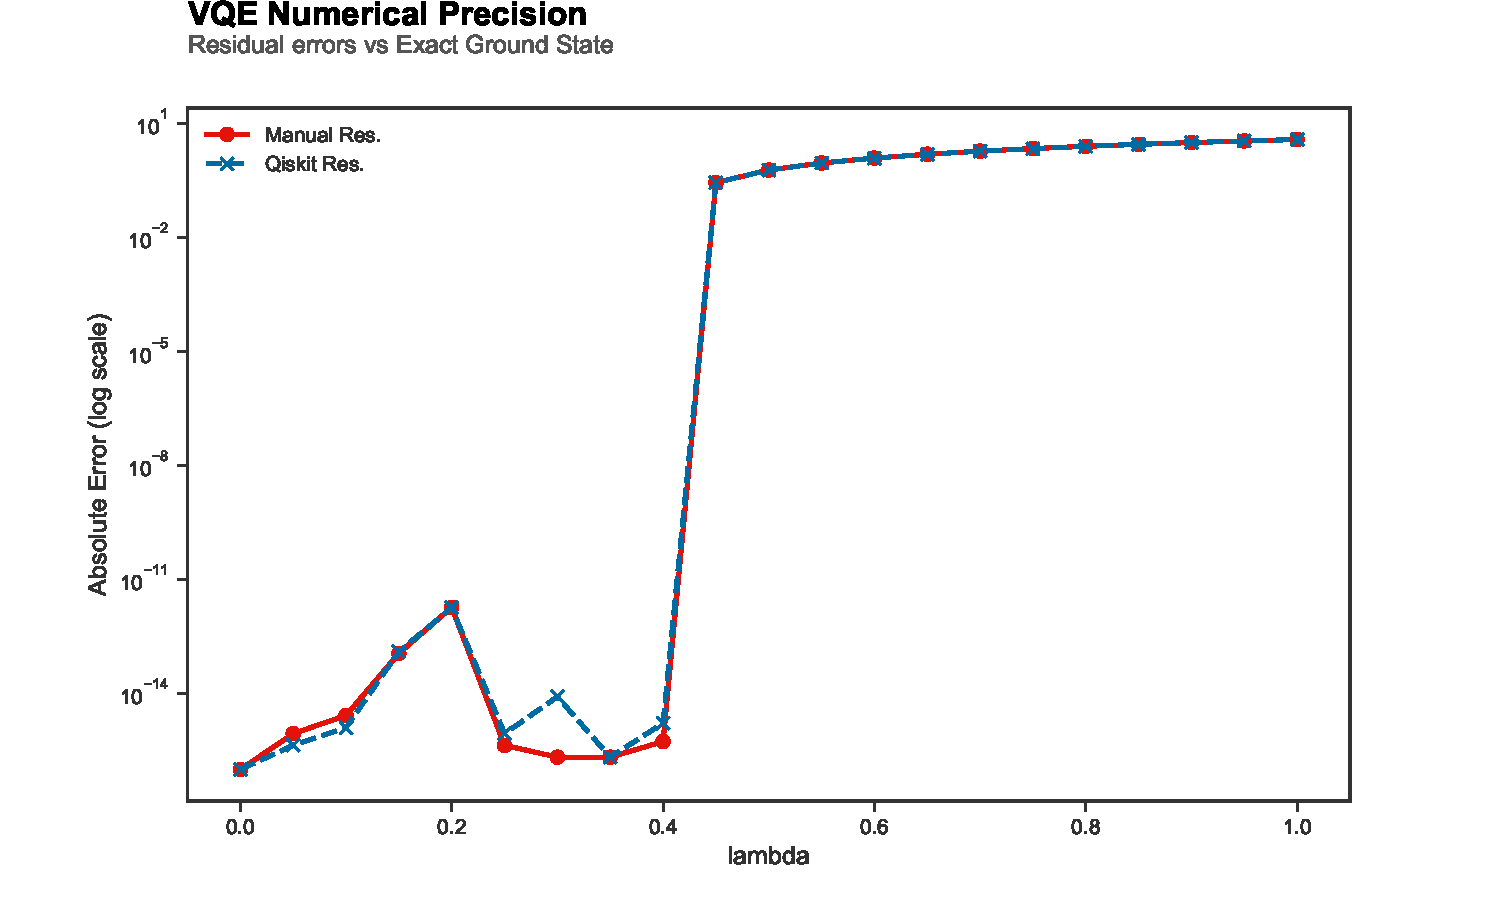
\includegraphics[width=\linewidth]{figures/part-e_vqe_precision.pdf}
\caption{Precision.}
\label{fig:app_e_prec}
\end{subfigure}
\caption{VQE performance for the two-qubit Hamiltonian.}
\label{fig:app_e}
\end{figure}

% \clearpage

% ---------- Part F ----------
\subsection*{Part F: Lipkin model (classical reference)}

\begin{figure}[H]
\centering
\begin{subfigure}[t]{0.4\textwidth}
\centering
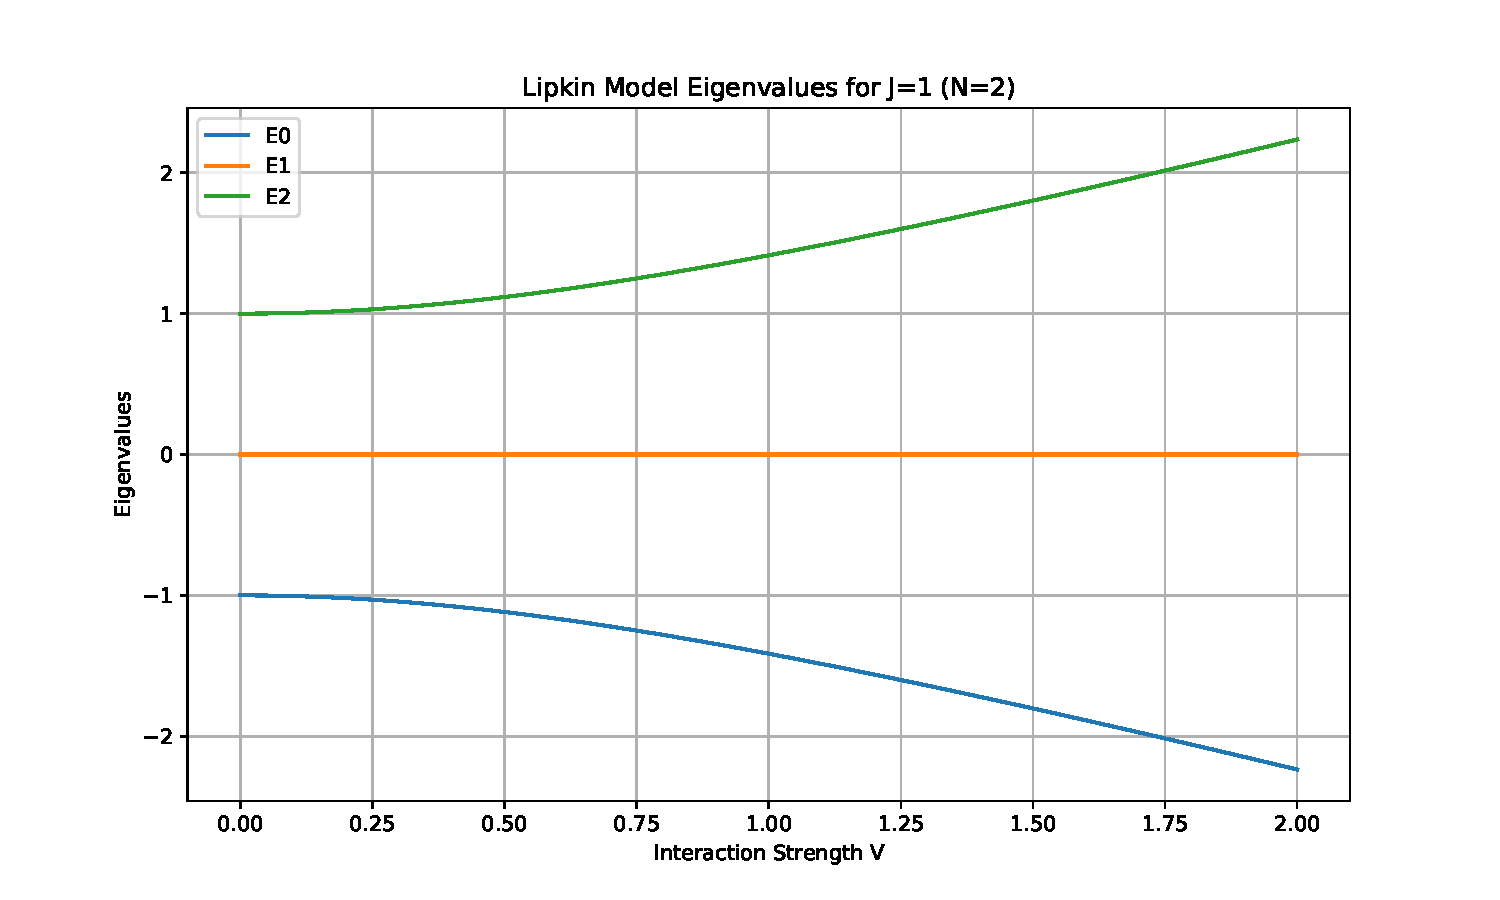
\includegraphics[width=\linewidth]{figures/part-f_j1.pdf}
\caption{$J=1$.}
\label{fig:app_f_j1}
\end{subfigure}
\hfill
\begin{subfigure}[t]{0.4\textwidth}
\centering
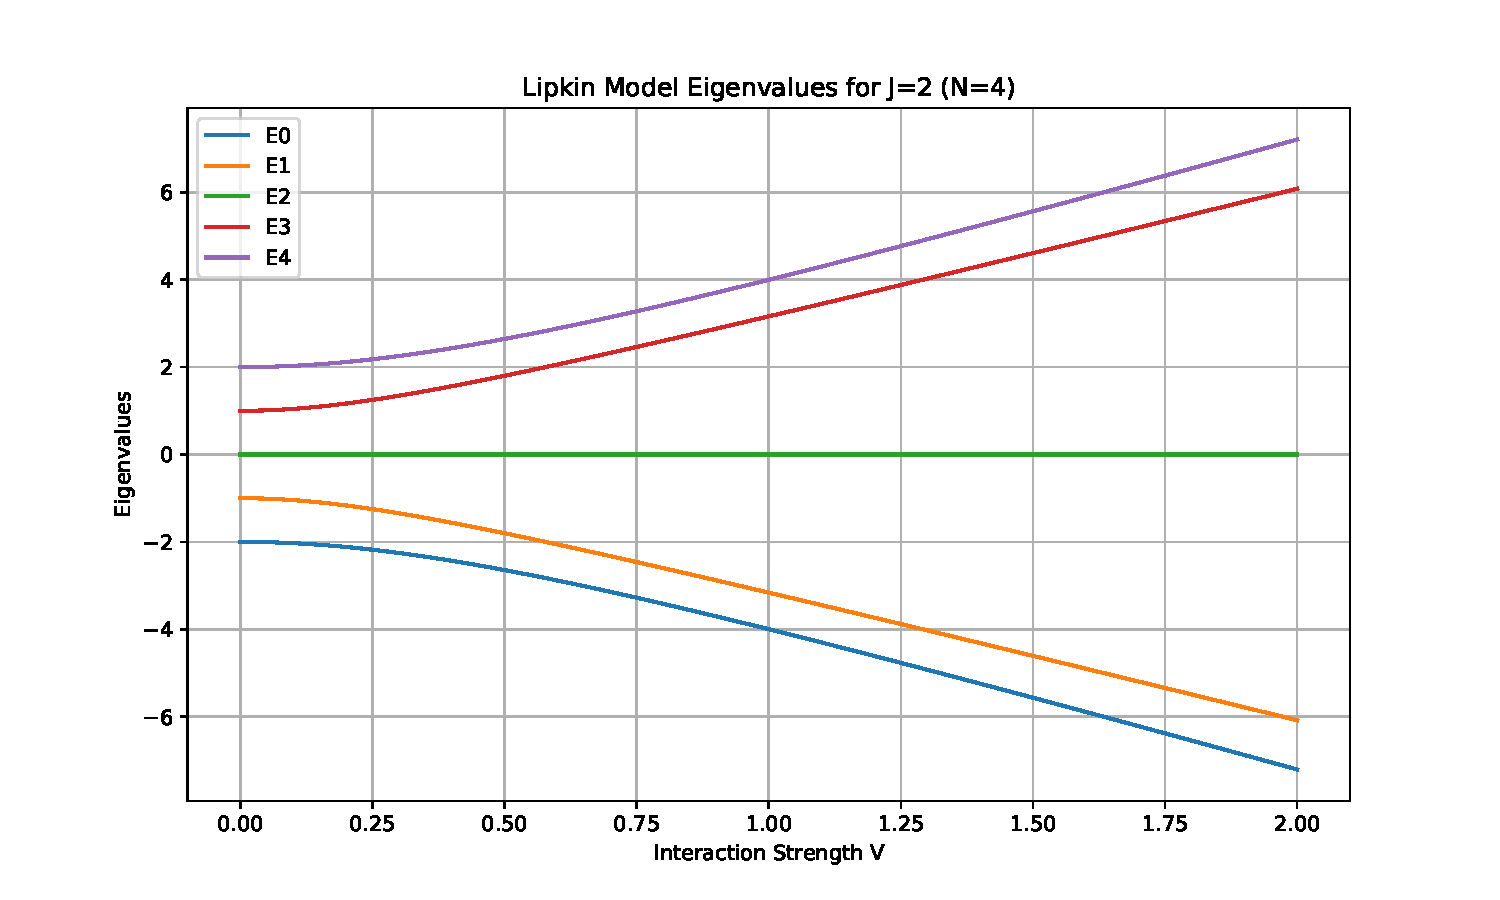
\includegraphics[width=\linewidth]{figures/part-f_j2.pdf}
\caption{$J=2$.}
\label{fig:app_f_j2}
\end{subfigure}

\vspace{0.6em}

\begin{subfigure}[t]{0.4\textwidth}
\centering
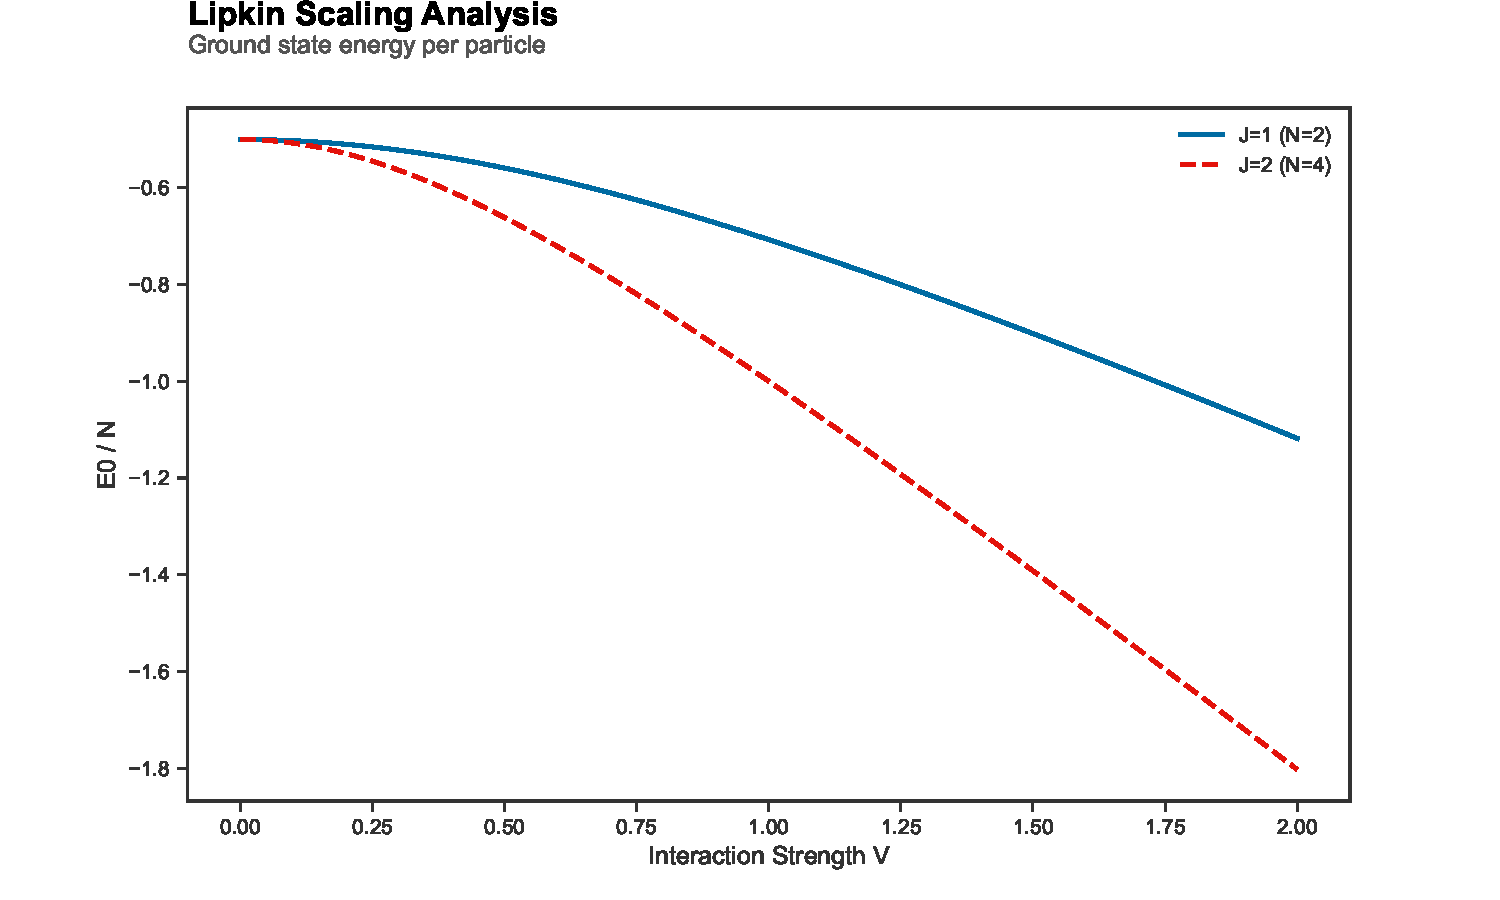
\includegraphics[width=\linewidth]{figures/part-f_scaling.pdf}
\caption{Scaling.}
\label{fig:app_f_scaling}
\end{subfigure}
\caption{Classical diagonalization results for the Lipkin model.}
\label{fig:app_f}
\end{figure}

% \clearpage

% ---------- Part G ----------
\subsection*{Part G: Lipkin model with VQE}

\begin{figure}[H]
\centering
\begin{subfigure}[t]{0.4\textwidth}
\centering
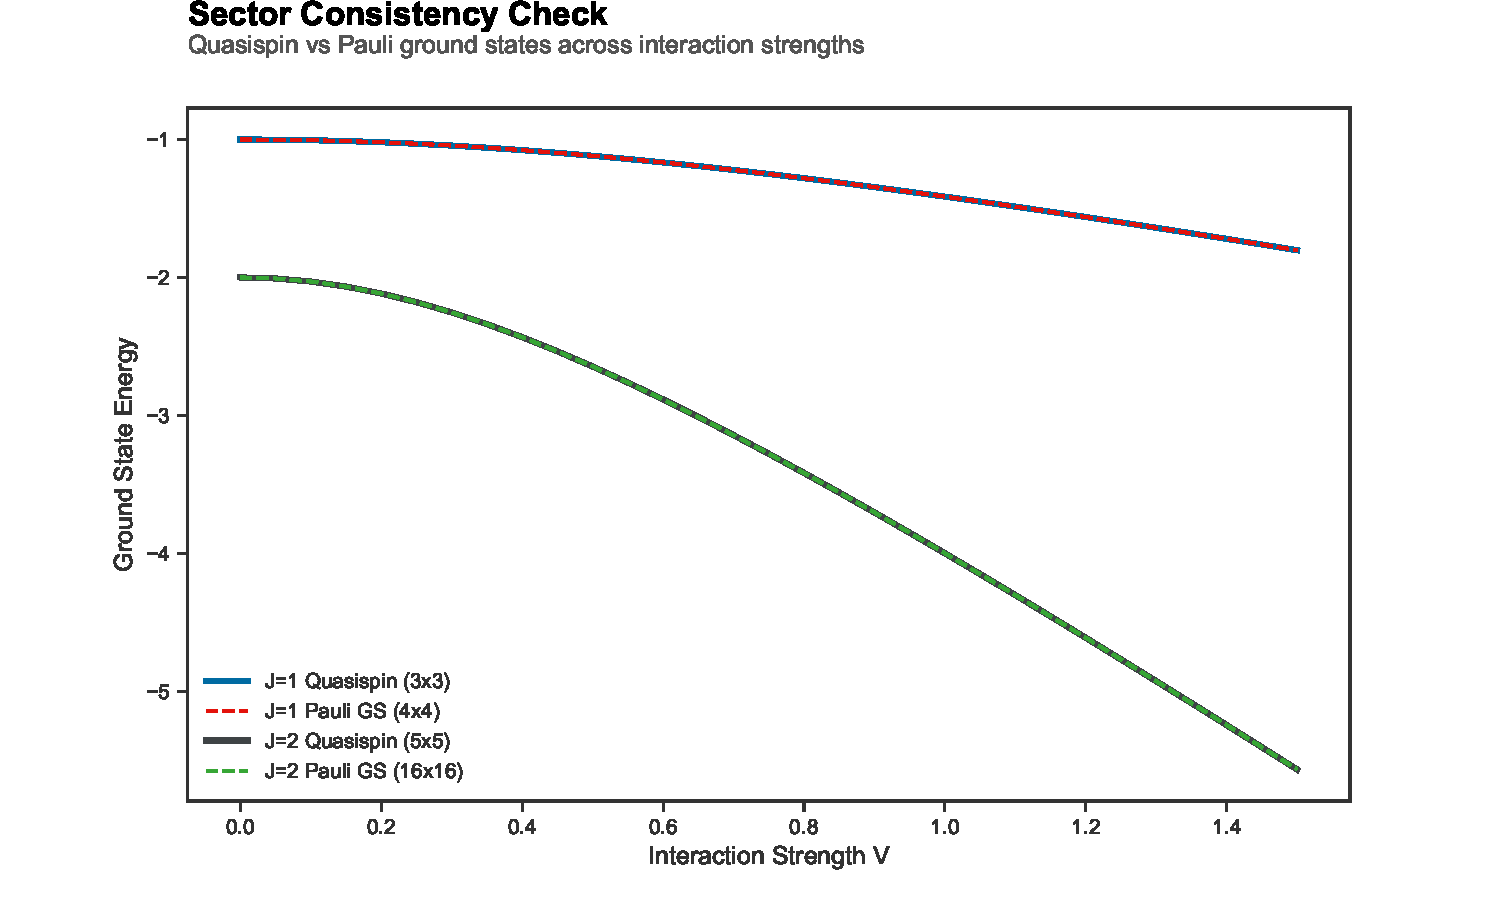
\includegraphics[width=\linewidth]{figures/part-g_sector_check.pdf}
\caption{Sector check.}
\label{fig:app_g_sector}
\end{subfigure}
\hfill
\begin{subfigure}[t]{0.4\textwidth}
\centering
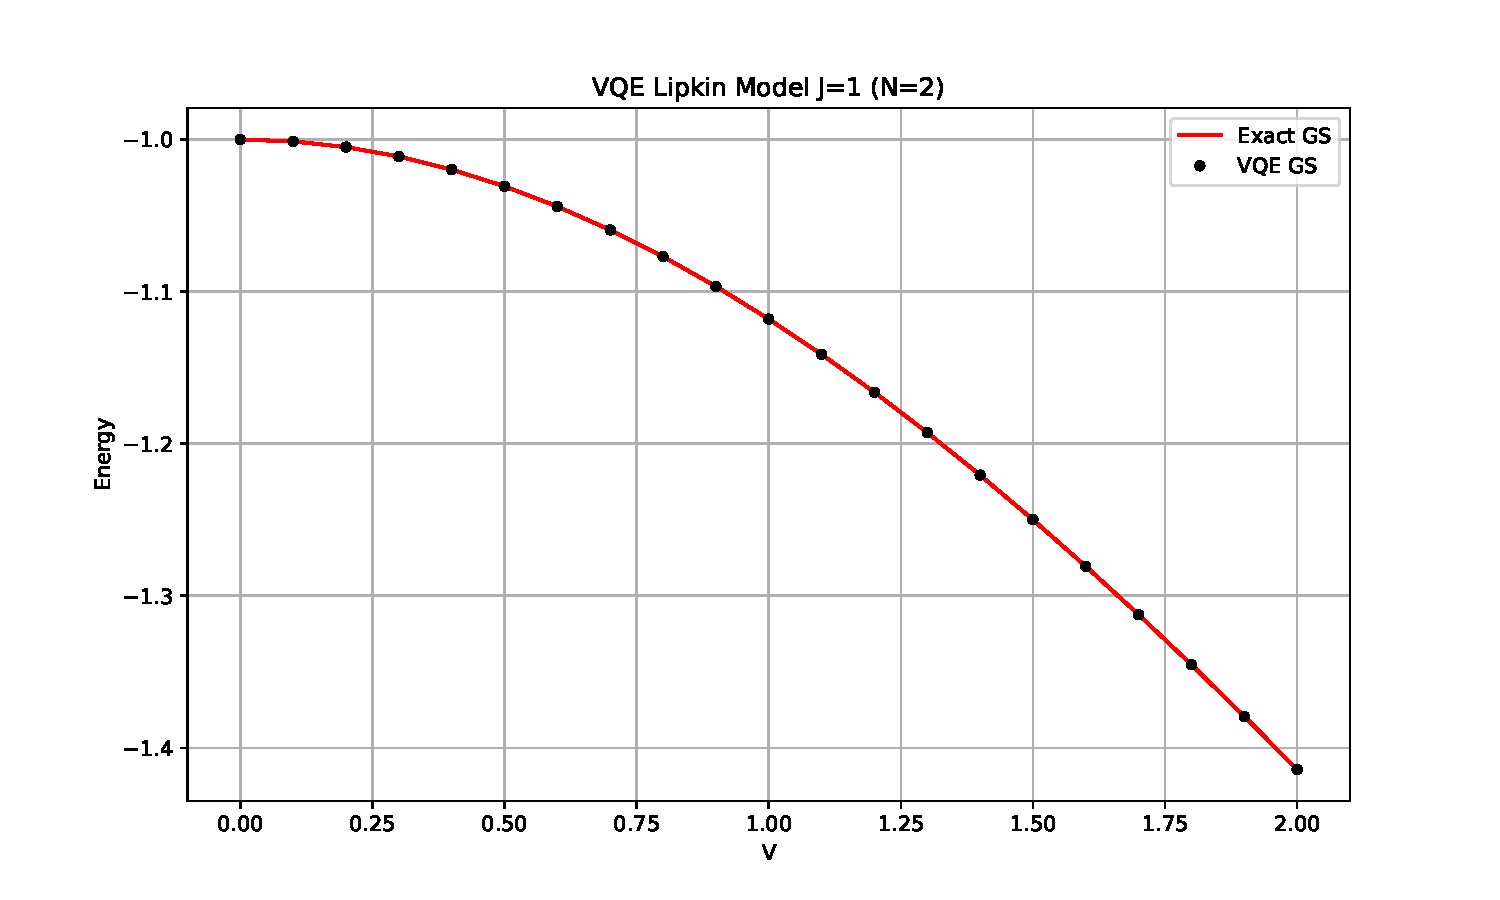
\includegraphics[width=\linewidth]{figures/part-g_vqe_j1.pdf}
\caption{VQE ($J=1$).}
\label{fig:app_g_j1}
\end{subfigure}

\vspace{0.6em}

\begin{subfigure}[t]{0.4\textwidth}
\centering
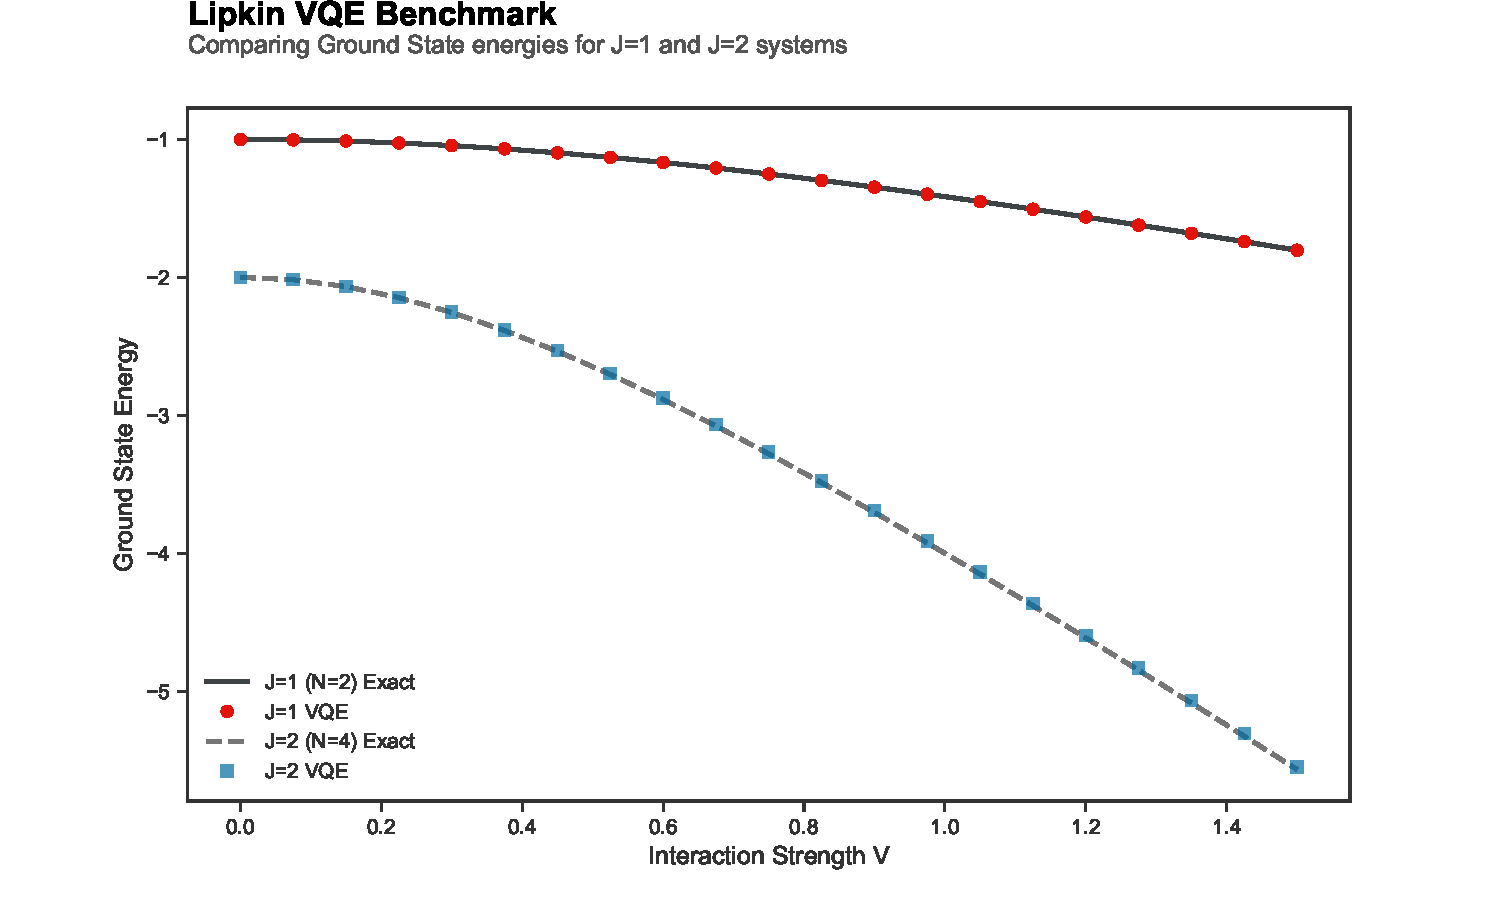
\includegraphics[width=\linewidth]{figures/part-g_vqe_manybody.pdf}
\caption{Many-body VQE.}
\label{fig:app_g_manybody}
\end{subfigure}
\hfill
\begin{subfigure}[t]{0.4\textwidth}
\centering
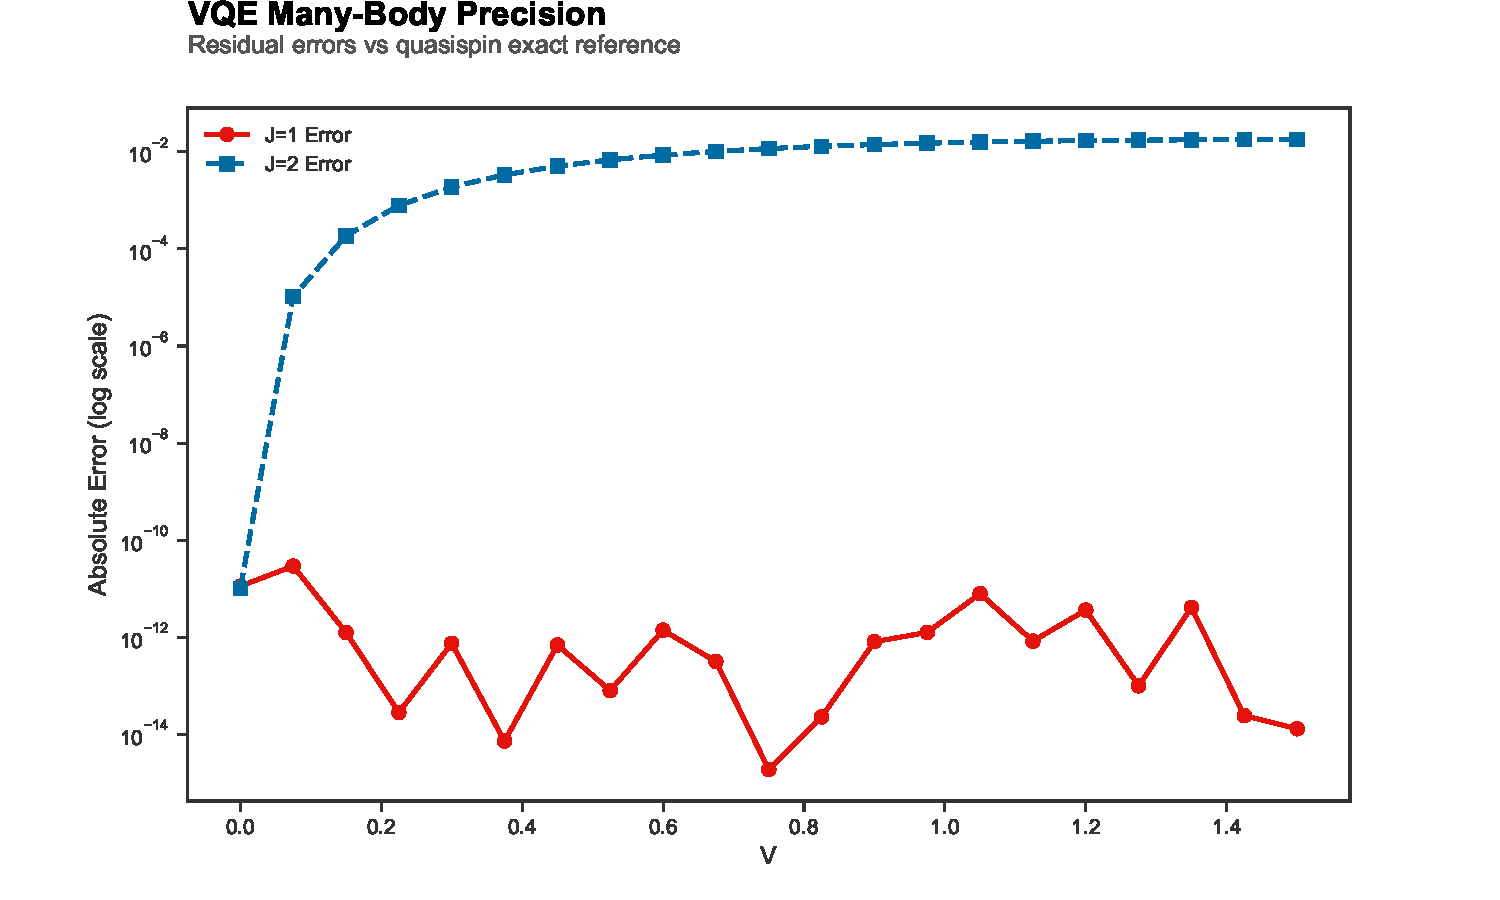
\includegraphics[width=\linewidth]{figures/part-g_vqe_precision.pdf}
\caption{Precision.}
\label{fig:app_g_prec}
\end{subfigure}
\caption{VQE diagnostics for the Lipkin model.}
\label{fig:app_g}
\end{figure}

\subsection{Programming with \texttt{python}}

\begin{lstlisting}[
captionpos=b,
caption={Python environment and core libraries used for the numerical simulations, classical diagonalization, and quantum-circuit implementations in this project. The environment includes scientific computing tools (NumPy, SciPy, pandas), visualization libraries (Matplotlib, Seaborn), and quantum computing frameworks (PennyLane and Qiskit).},
label={lst:python-environment}
]
absl-py>=2.1.0
cplex>=22.1.2.0
gurobipy>=13.0.1
hmmlearn>=0.3.3
matplotlib>=3.7.1
nautilus_trader>=1.155.0
numpy>=1.24.3
pandas>=2.2.2
pennylane>=0.38.0
pyarrow>=17.0.0
pylatexenc>=2.10
qiskit>=1.0.0
qiskit-aer>=0.17.2
qiskit-algorithms>=0.4.0
qiskit-ibm-runtime>=0.45.1
qiskit-optimization>=0.7.0
scipy>=1.14.1
seaborn>=0.13.2
sympy>=1.13.3
vectorbt>=0.26.0
\end{lstlisting}